\section{Bode e Nyquist}
\label{sec:bode_nyquist}
%===============================================================================

Nesta se��o ser� apresentado o diagrama de Bode e Nyquist para o processo, descrito 
em (\ref{fig:intro_sistema}). Utilizando-se duas abordagens: 

\begin{itemize}
\item B�sico onde aplica-se um onda senoidal na entrada do processo e mede-se a amplitude
e a fase da onda que foi produzida na sa�da.

\item M�todo melhorado, onde tenta-se reduzir a influ�ncia do ruido sobre as medidas coletadas.

\end{itemize}

A fim de comparar os resultados obtidos com um resultado correto, foi apresentado nas
Figuras (\ref{fig:bode_sem_ruido}) e  (\ref{fig:nyquist_sem_ruido}) os diagramas de 
Bode e Nyquist respectivamente do sistema sem ruido. Nas abordagens seguintes o sistema 
considerado ter� ruido e ser� feito um comparativo para determinar qual m�todo se aproxima
mais da resposta real do sistema.

\begin{figure}[htbp]
	\center
	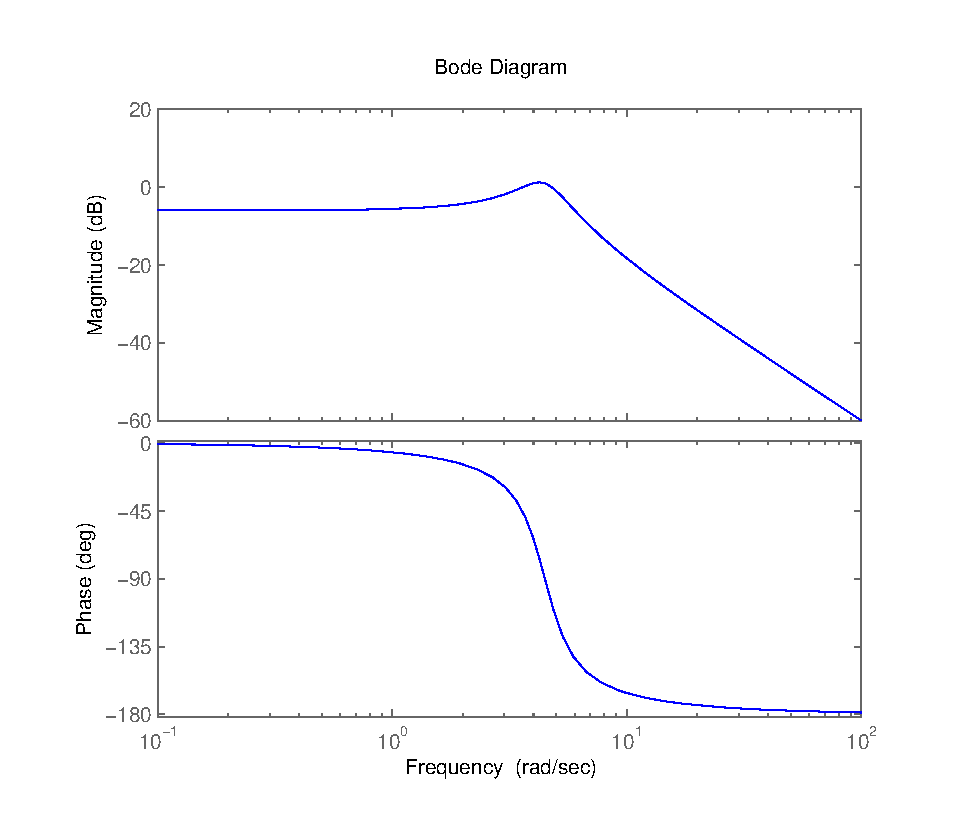
\includegraphics[width=0.98\columnwidth]{figures/bode_sem_ruido.eps}
	\caption{Diagrama de bode do sistema sem ruido.}
	\label{fig:bode_sem_ruido}
\end{figure}

\begin{figure}[htbp]
	\center
	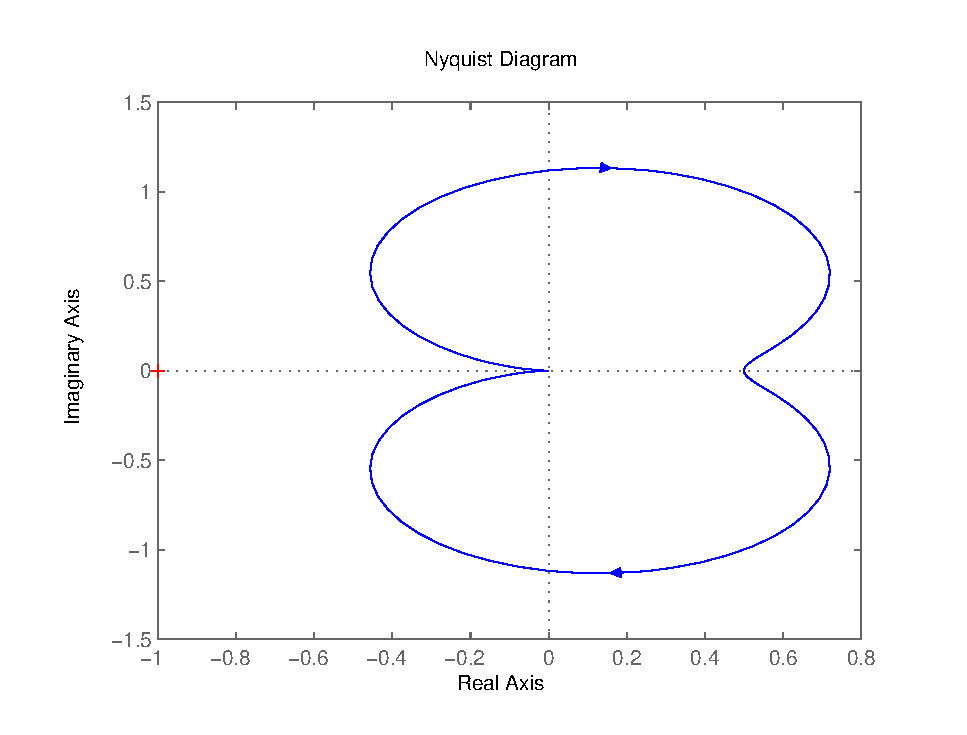
\includegraphics[width=0.98\columnwidth]{figures/nyquist_sem_ruido.eps}
	\caption{Diagrama de Nyquist do sistema sem ruido.}
	\label{fig:nyquist_sem_ruido}
\end{figure}

%===============================================================================
\subsection{M�todo B�sico}
\label{sec:bode_nyquest_basico}

Este m�todo simples consiste em aplicar uma onda senoidal na entrada do processo e observar qual
� a defasagem que a planta imp�em sobre a onde da entrada e a qual � o ganho de amplitude que 
� aplicado.

Como a planta em quest�o possui ru�do aditivo na sa�da, tem-se que as medidas efetuadas por este
m�todo s�o muito imprecisas, para calcular a amplitude do sinal de saida, basta analisar um ponto
que fique mediano ao ruido observado, mas para a fase, esta informa��o � mais complicada, pois como
a defasagem na planta em estudo � pequena, o ruido � muito grande, proporcionalmente, tornando as
medidas muito incertas.

Na Figura (\ref{fig:basic_method_1}) apresenta-se uma resposta padr�o para uma entrada senoidal.
Observa-se que a sa�da possui um ruido significante. Utilizando-se o mesmo procedimento, para diversas
frequencias de ondas senoidais na entrada do processo, obt�m-se diversos pontos do diagrama de 
resposta em frequencia do processo.

\begin{figure}[htbp]
	\center
	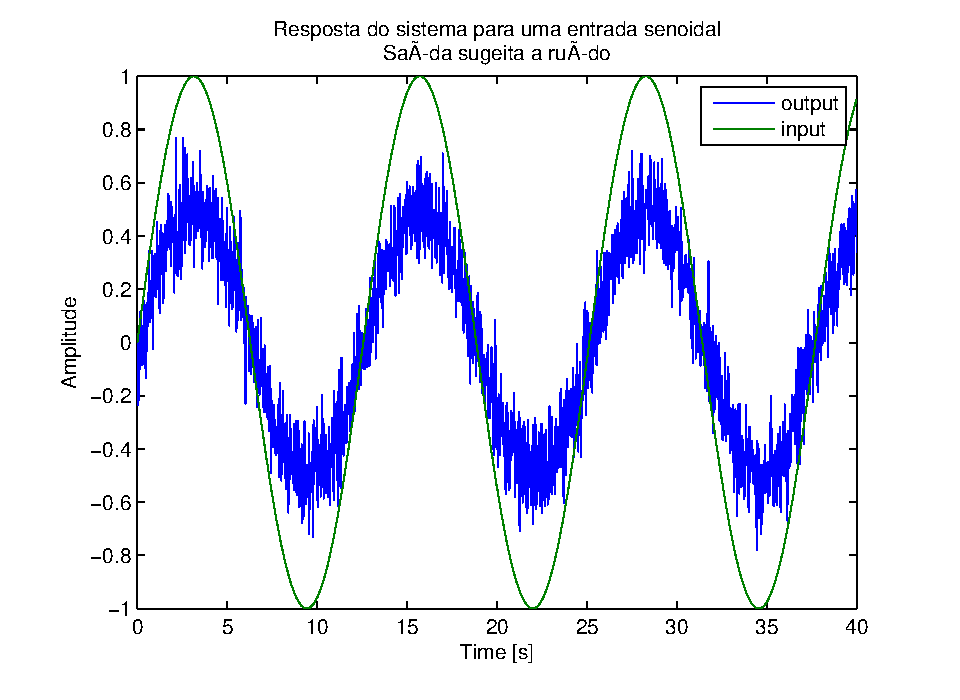
\includegraphics[width=0.98\columnwidth]{figures/basic_method_1.eps}
	\caption{Resposta do sistema para entrada senoidal}
	\label{fig:basic_method_1}
\end{figure}

Esta informa��es coletadas sobre o ganho e o deslocamento de fase aplicado sobre o sistema, chega-se as
informa��es que est�o contidas na Tabela (\ref{tab:basic_method})

\begin{table}[htbp]
  \begin{center}
	\caption{M�todo b�sico}
	\label{tab:basic_method}
	\begin{small}
	  \begin{tabular}{cll}
		\hline
		Frequ�ncia			& Ganho			& Fase [deg]	\\
		\hline
		0.01				& 0.5			& 0				\\
		0.1					& 0.45			& -11			\\
		0.5					& 0.5			& -46			\\
		1					& 0.55			& -14			\\
		5					& 0.85			& -86			\\
		10					& 0.14			& -200			\\
		50					& 0.13			& -186			\\
		100					& 0.0008		& -183			\\
		\hline
	  \end{tabular}
	\end{small}
  \end{center}
\end{table}

Os dados apresentados na Tabela (\ref{tab:basic_method}), podem ser utilizados para a confec��o 
do diagrama de bode do sistema apresentado na Figura (\ref{fig:bode_basic_method}). Observa-se que o formato
das curvas de fase e magnitude lembram as da Figura (\ref{fig:bode_sem_ruido}), mas a curva n�o
possui um fidelidade com a que caracteriza o sistema sem perturba��o.

\begin{figure}[htbp]
	\center
	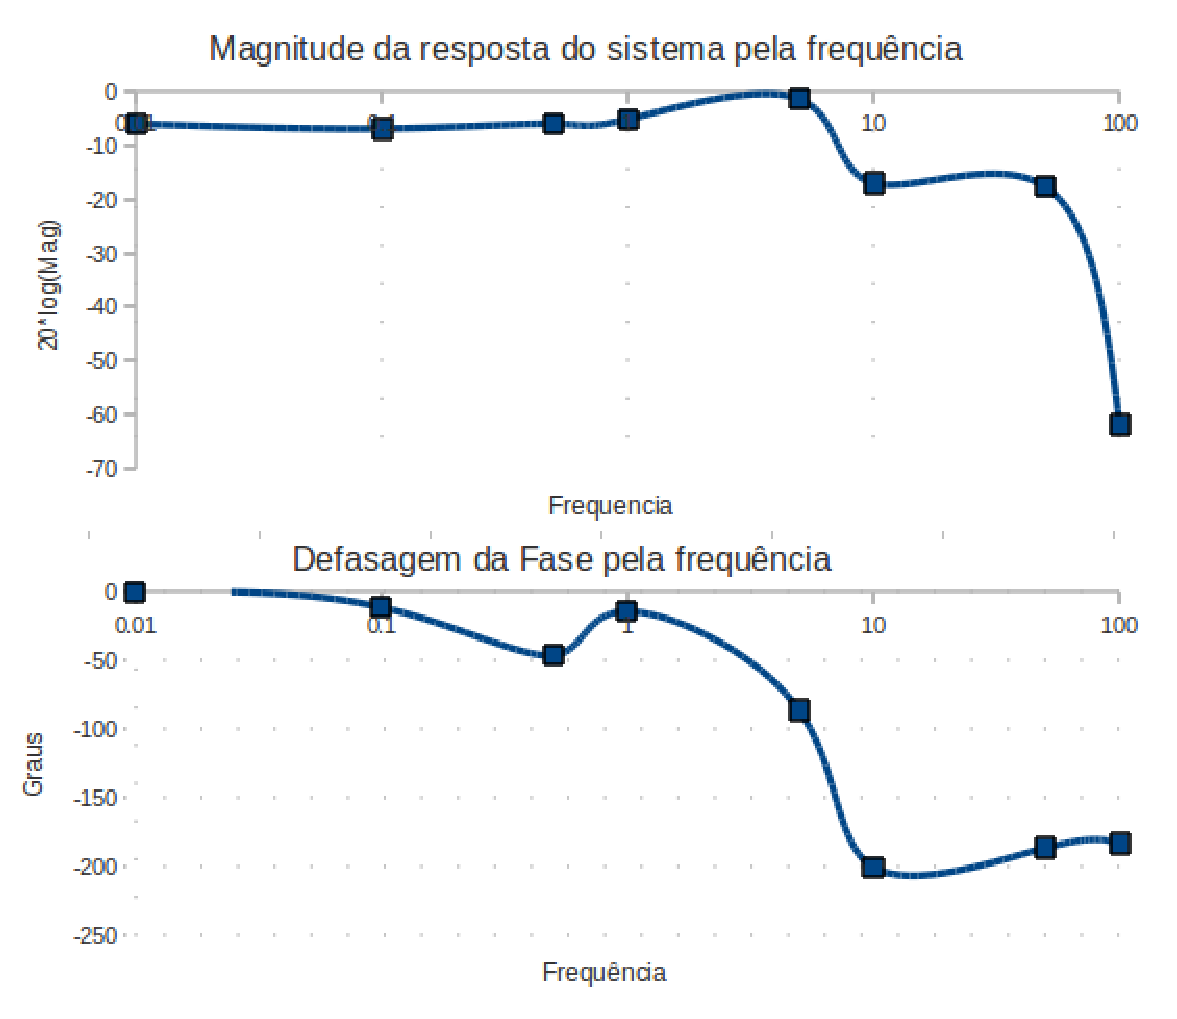
\includegraphics[width=0.98\columnwidth]{figures/basic_method.eps}
	\caption{Diagrama de Bode para o sistema sujeito a ruido, utilizando-se o m�todo b�sico para a 
	identifica��o da curva de resposta em frequ�ncia.}
	\label{fig:bode_basic_method}
\end{figure}
%===============================================================================
\subsection{M�todo melhorado}
\label{sec:bode_nyquest_melhorado}

